%%%%%%%%%%%%%%%%%%%%%%%%%%%%%%%%%%%%%%%%%%%%%%%%%%%%%%%%%%%%%%%%%%%%%%%%%%%%%%%%%
\section{Scalar Results}
%%%%%%%%%%%%%%%%%%%%%%%%%%%%%%%%%%%%%%%%%%%%%%%%%%%%%%%%%%%%%%%%%%%%%%%%%%%%%%%%%
\begin{frame}
\frametitle{Source-in-Absorber Test Problem}
\framesubtitle{Strong Absorber with Source in Left Half of Domain, FE}

\begin{center}
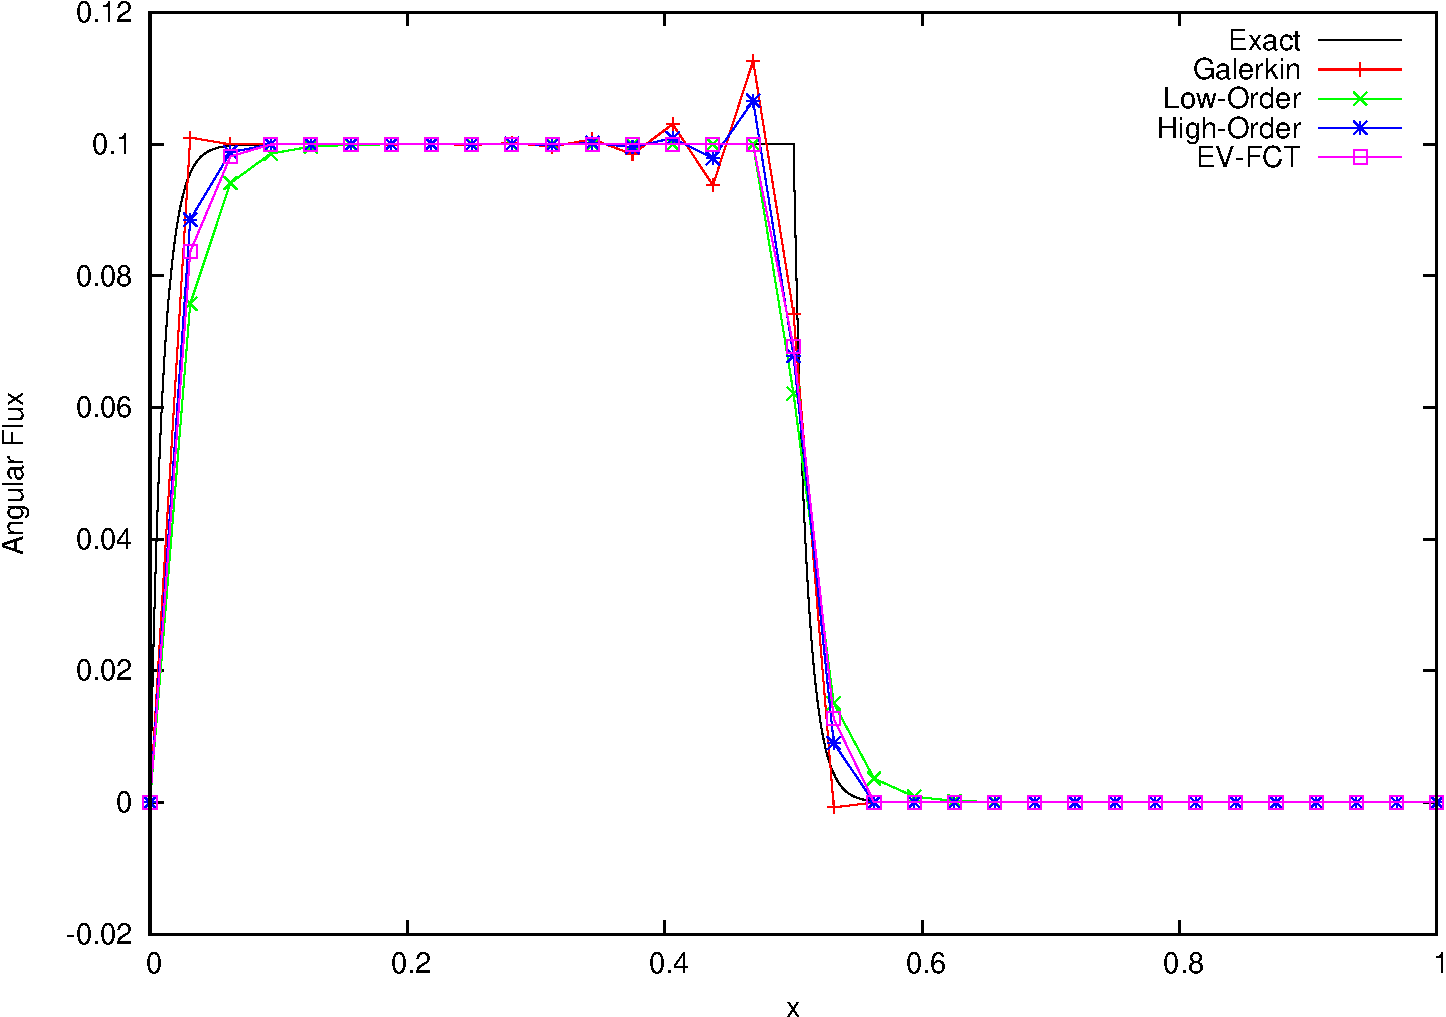
\includegraphics[height=0.8\textheight]{./figures/solutions_source_FE.pdf}
\end{center}

\end{frame}
%%%%%%%%%%%%%%%%%%%%%%%%%%%%%%%%%%%%%%%%%%%%%%%%%%%%%%%%%%%%%%%%%%%%%%%%%%%%%%%%%
\begin{frame}
\frametitle{2-D Void-to-Absorber Test Problem}
\framesubtitle{Normally-Incident Wave from Void to Absorber Quadrant, FE}

\begin{figure}[h]
   \centering
   \begin{subfigure}{0.3\textwidth}
      \centering
      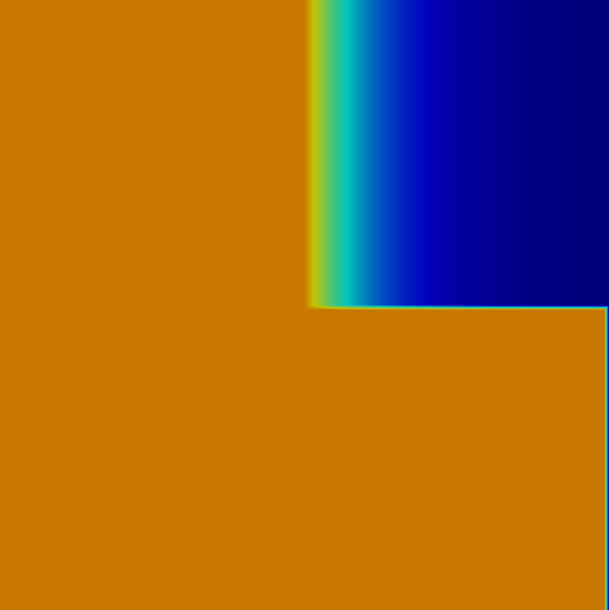
\includegraphics[width=0.8\textwidth]{./figures/exact.png}
      \caption{Exact}
   \end{subfigure}
   \begin{subfigure}{0.3\textwidth}
      \centering
      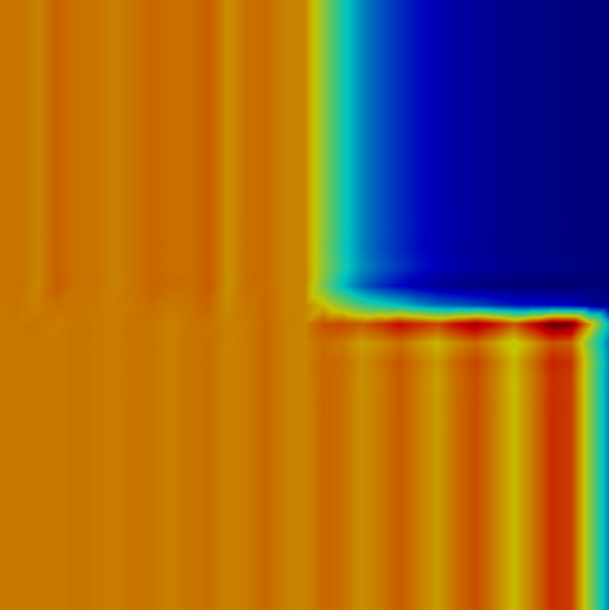
\includegraphics[width=0.8\textwidth]{./figures/Gal.png}
      \caption{Galerkin}
   \end{subfigure}
   \begin{subfigure}{0.3\textwidth}
      \centering
      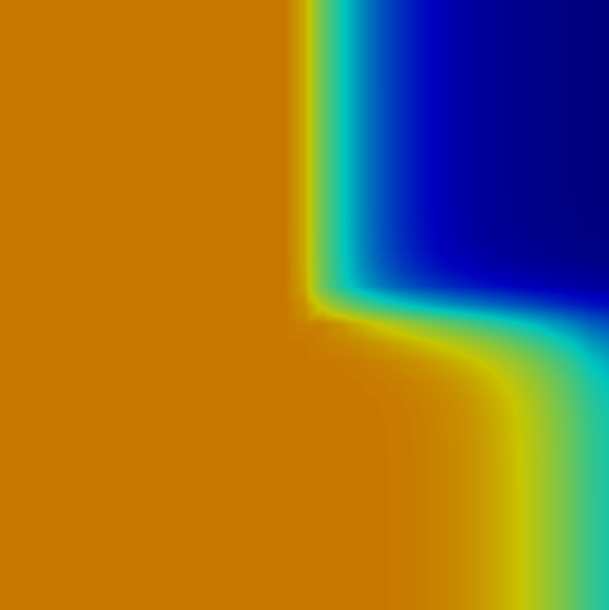
\includegraphics[width=0.8\textwidth]{./figures/GalFCT.png}
      \caption{Galerkin-FCT}
   \end{subfigure}
   \begin{subfigure}{0.3\textwidth}
      \centering
      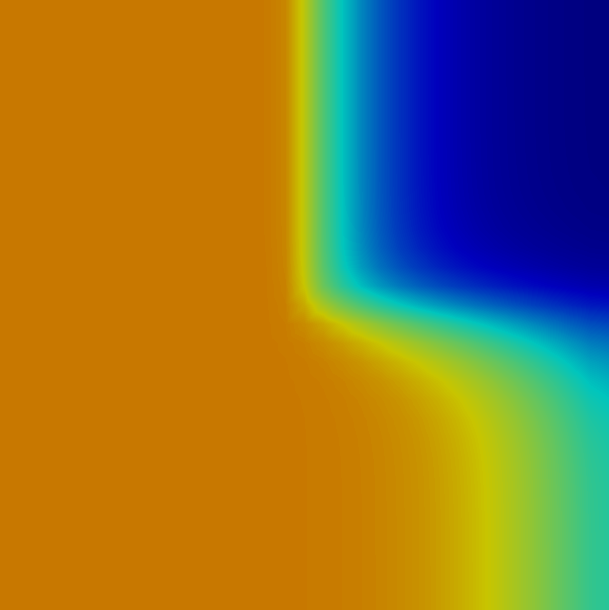
\includegraphics[width=0.8\textwidth]{./figures/low.png}
      \caption{Low-order}
   \end{subfigure}
   \begin{subfigure}{0.3\textwidth}
      \centering
      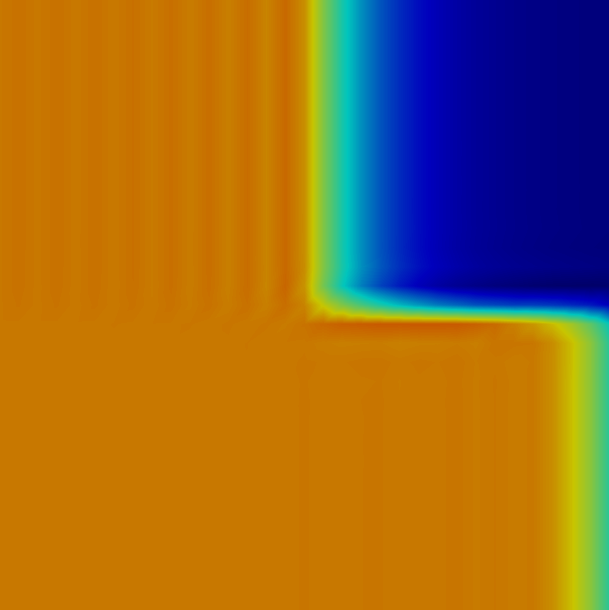
\includegraphics[width=0.8\textwidth]{./figures/EV.png}
      \caption{EV}
   \end{subfigure}
   \begin{subfigure}{0.3\textwidth}
      \centering
      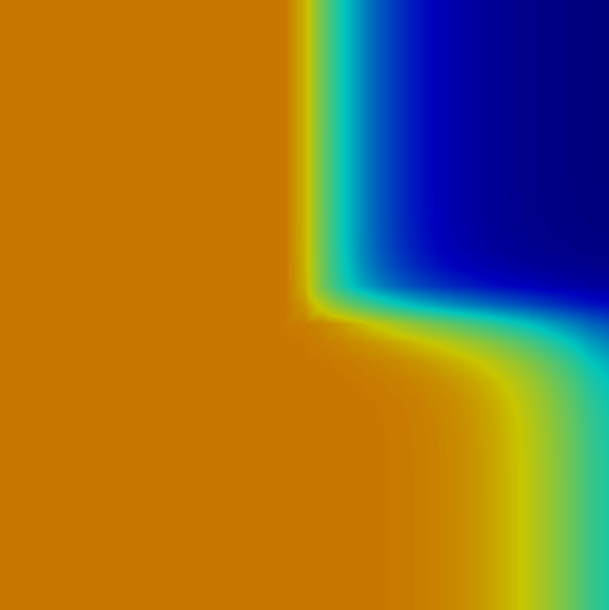
\includegraphics[width=0.8\textwidth]{./figures/EVFCT.png}
      \caption{EV-FCT}
   \end{subfigure}
\end{figure}

\end{frame}
%%%%%%%%%%%%%%%%%%%%%%%%%%%%%%%%%%%%%%%%%%%%%%%%%%%%%%%%%%%%%%%%%%%%%%%%%%%%%%%%%
\begin{frame}
\frametitle{1-D Smooth Problem Convergence Test}
\framesubtitle{MMS Solution: $u(x,t)=t\sin(\pi x)$, FE}

\begin{center}
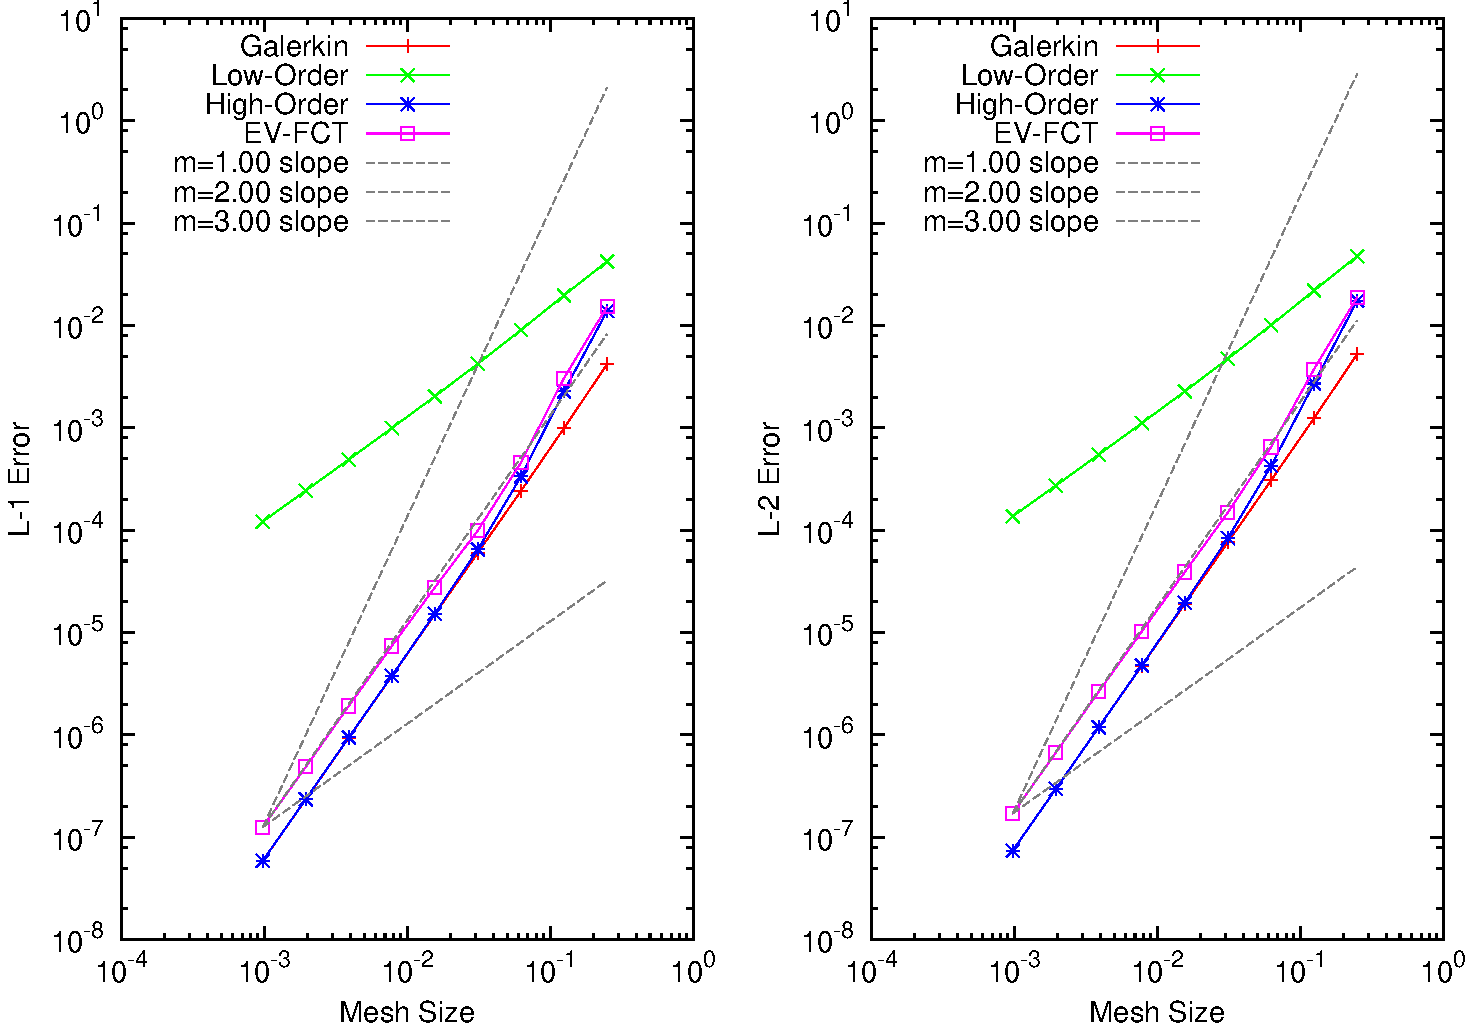
\includegraphics[height=0.8\textheight]{./figures/convergence_smooth_FE.pdf}
\end{center}

\end{frame}
%%%%%%%%%%%%%%%%%%%%%%%%%%%%%%%%%%%%%%%%%%%%%%%%%%%%%%%%%%%%%%%%%%%%%%%%%%%%%%%%%
\begin{frame}
\frametitle{1-D Non-smooth Problem Convergence Test}
\framesubtitle{Linear Advection of Discontinuous Wave Front, SSPRK33}

\begin{center}
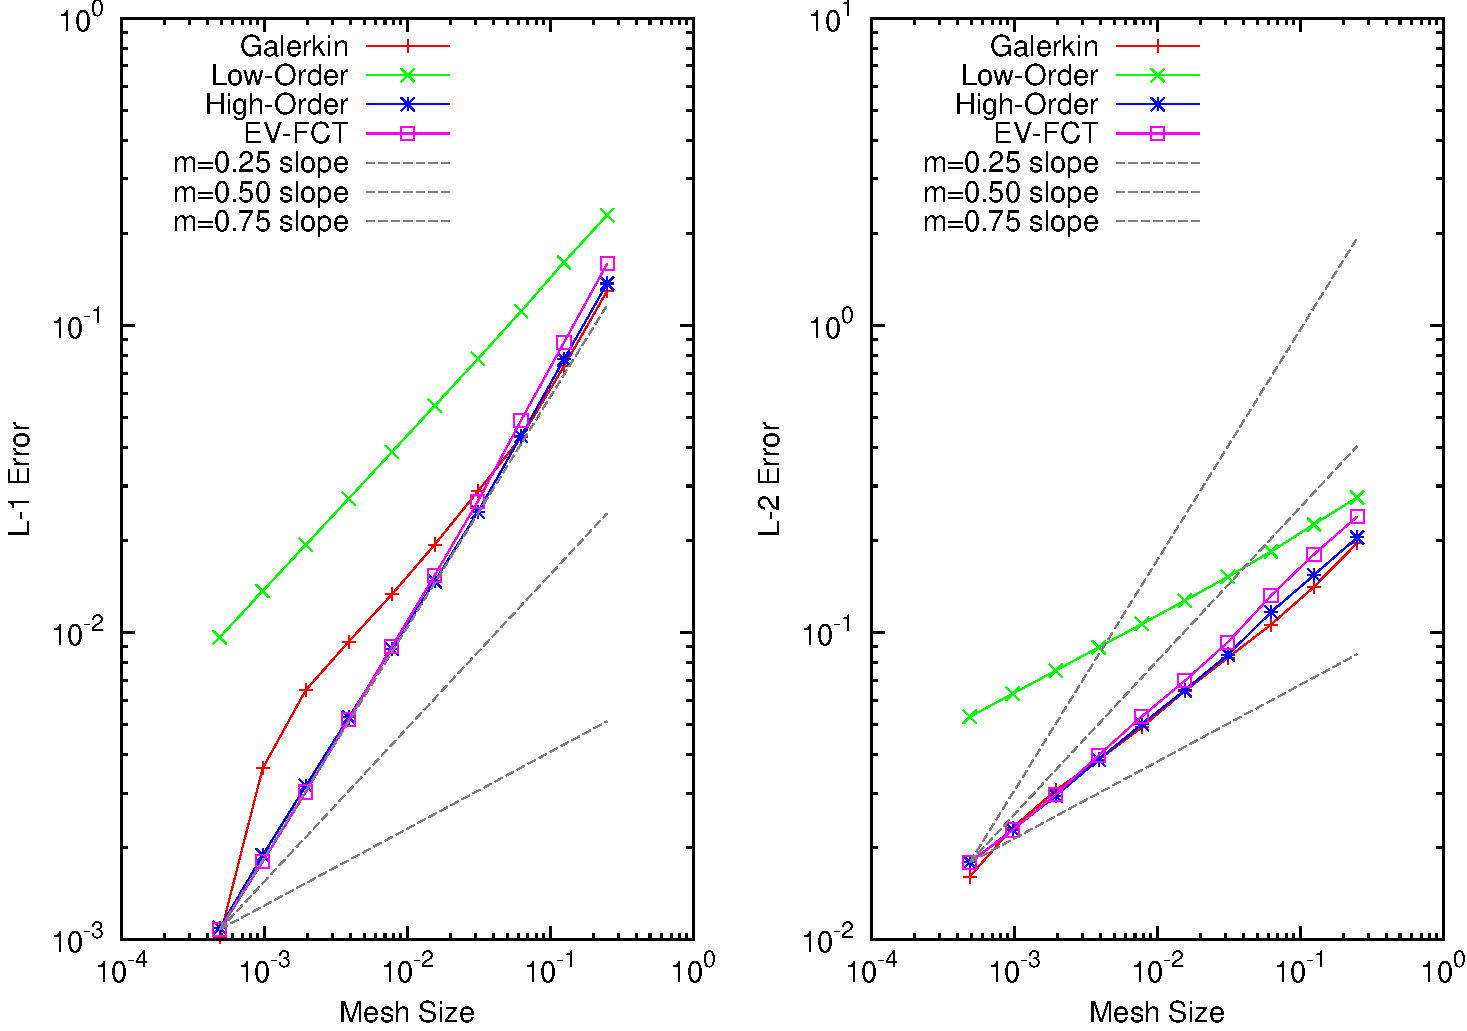
\includegraphics[height=0.8\textheight]{./figures/convergence_absorber_SSPRK33.pdf}
\end{center}

\end{frame}
%%%%%%%%%%%%%%%%%%%%%%%%%%%%%%%%%%%%%%%%%%%%%%%%%%%%%%%%%%%%%%%%%%%%%%%%%%%%%%%%%
\begin{frame}
\frametitle{Obstruction Test Problem}
\framesubtitle{$45^\circ$-degree Flux Incident on Square Absorber Region, 4096 cells, FE}

\begin{figure}[h]
   \centering
   \begin{subfigure}{0.49\textwidth}
      \centering
      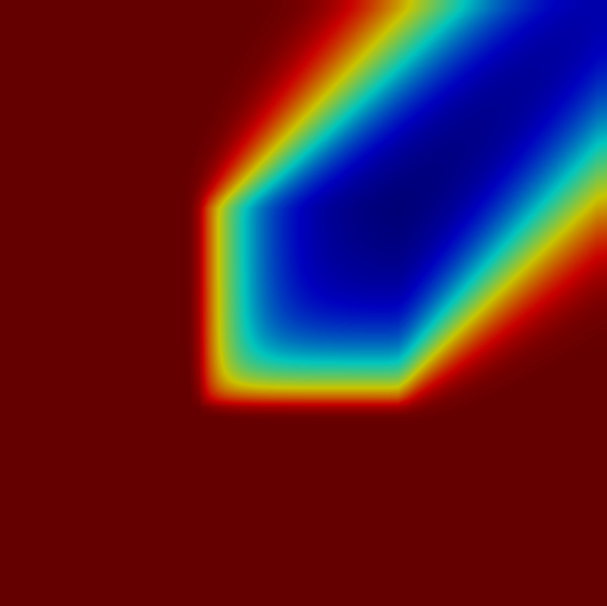
\includegraphics[width=\textwidth]{./figures/obstruction_Low_FE.png}
      \caption{Low-order}
   \end{subfigure}
   \begin{subfigure}{0.49\textwidth}
      \centering
      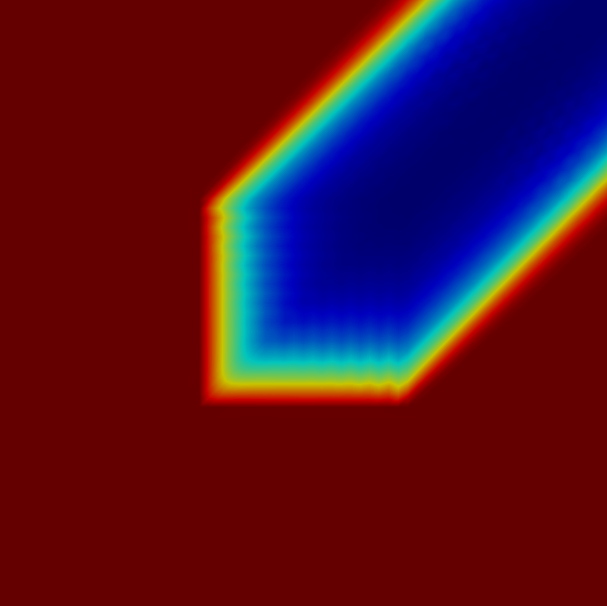
\includegraphics[width=\textwidth]{./figures/obstruction_EVFCT_FE.png}
      \caption{EV-FCT}
   \end{subfigure}
\end{figure}

\end{frame}
%%%%%%%%%%%%%%%%%%%%%%%%%%%%%%%%%%%%%%%%%%%%%%%%%%%%%%%%%%%%%%%%%%%%%%%%%%%%%%%%%
\begin{frame}
\frametitle{Obstruction Test Problem}
\framesubtitle{CFL Number vs. Iterations Study, Backward Euler, 256 cells}

\begin{center}
\begin{table}[h]
\caption{EV and FCT Iterations Required for EV-FCT Solution}
\begin{tabular}{c c c c c}\toprule
\emph{CFL} & \multicolumn{2}{c}{\emph{EV}} & \multicolumn{2}{c}{\emph{FCT}}\\
           & \emph{Total} & \emph{Avg.}    &  \emph{Total} & \emph{Avg.}\\\midrule
0.1  & 3999 &  8.14 & 3585 &   7.30\\
0.5  &  896 &  9.05 & 1499 &  15.14\\
1.0  &  501 & 10.02 &  970 &  19.40\\
5.0  &  157 & 15.70 & 1130 & 113.00\\
10.0 &   79 & 15.80 &  753 & 150.60\\
20.0 &   -- &    -- & \multicolumn{2}{c}{\textcolor{red}{\textbf{FAIL}}}\\
\bottomrule\end{tabular}
\end{table}
\end{center}

\end{frame}
%%%%%%%%%%%%%%%%%%%%%%%%%%%%%%%%%%%%%%%%%%%%%%%%%%%%%%%%%%%%%%%%%%%%%%%%%%%%%%%%%
\begin{frame}
\frametitle{Glance-in-Void Test Problem}
\framesubtitle{Glancing Incident Flux in a Vacuum, 4096 cells}

\begin{figure}[h]
   \centering
   \begin{subfigure}{0.3\textwidth}
      \centering
      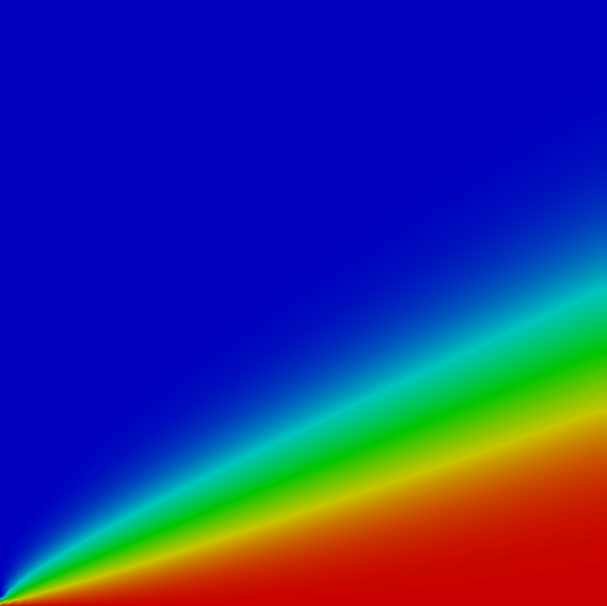
\includegraphics[width=0.8\textwidth]{./figures/glance_DMP_FE.png}
      \caption{Low-order, FE}
   \end{subfigure}
   \begin{subfigure}{0.3\textwidth}
      \centering
      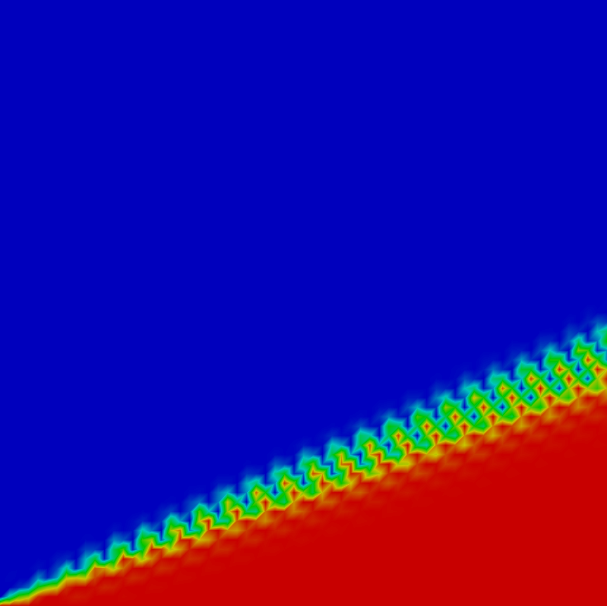
\includegraphics[width=0.8\textwidth]{./figures/glance_GalFCT_FE.png}
      \caption{Gal-FCT, FE}
   \end{subfigure}
   \begin{subfigure}{0.3\textwidth}
      \centering
      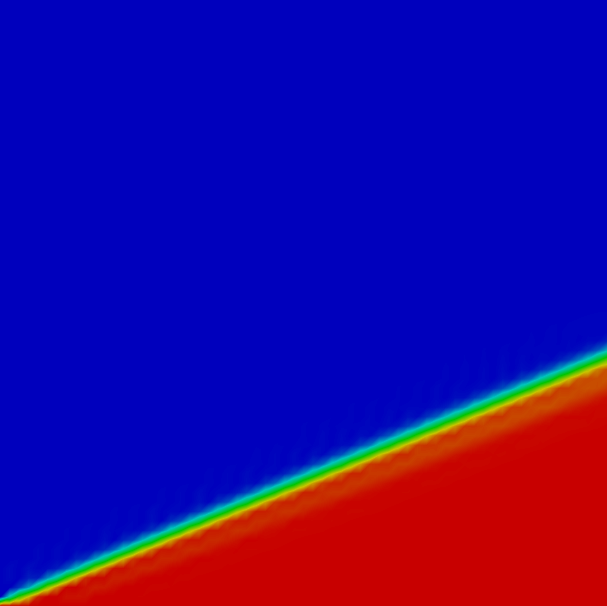
\includegraphics[width=0.8\textwidth]{./figures/glance_GalFCT_SSP3.png}
      \caption{Gal-FCT, SSPRK33}
   \end{subfigure}
   \begin{subfigure}{0.3\textwidth}
      \centering
      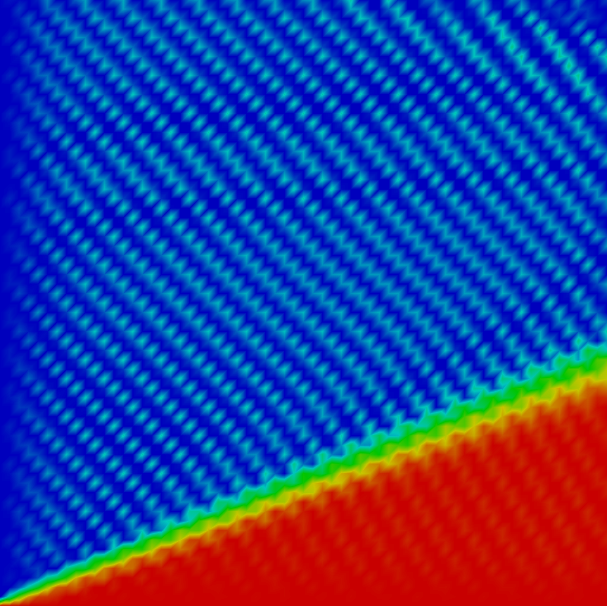
\includegraphics[width=0.8\textwidth]{./figures/glance_EV_FE_cE01.png}
      \caption{EV, FE}
   \end{subfigure}
   \begin{subfigure}{0.3\textwidth}
      \centering
      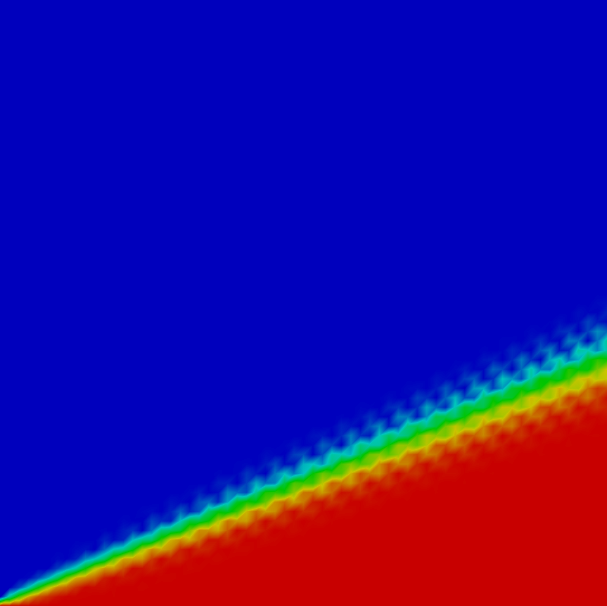
\includegraphics[width=0.8\textwidth]{./figures/glance_EVFCT_FE_cE01.png}
      \caption{EV-FCT, FE}
   \end{subfigure}
   \begin{subfigure}{0.3\textwidth}
      \centering
      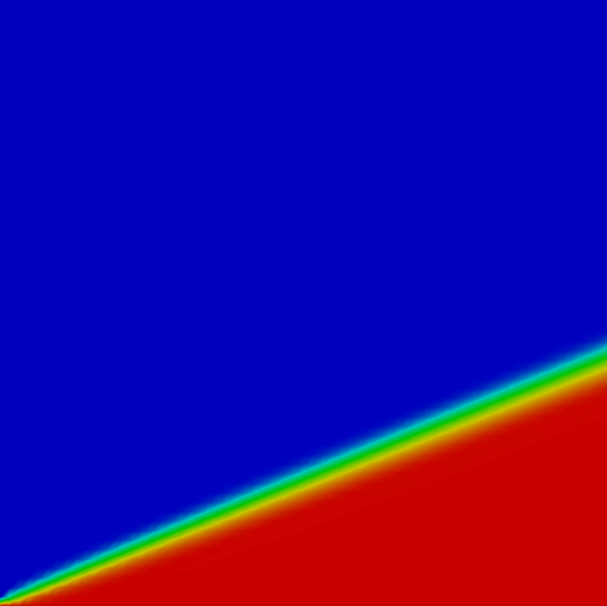
\includegraphics[width=0.8\textwidth]{./figures/glance_EVFCT_SSP3_cE01.png}
      \caption{EV-FCT, SSPRK33}
   \end{subfigure}
\end{figure}

\end{frame}
%%%%%%%%%%%%%%%%%%%%%%%%%%%%%%%%%%%%%%%%%%%%%%%%%%%%%%%%%%%%%%%%%%%%%%%%%%%%%%%%%
\begin{frame}
\frametitle{Source-Void-to-Absorber Test Problem}
\framesubtitle{Strongly Imposed Dirichlet BC, $L^+=L^-=1$, SS}

\begin{center}
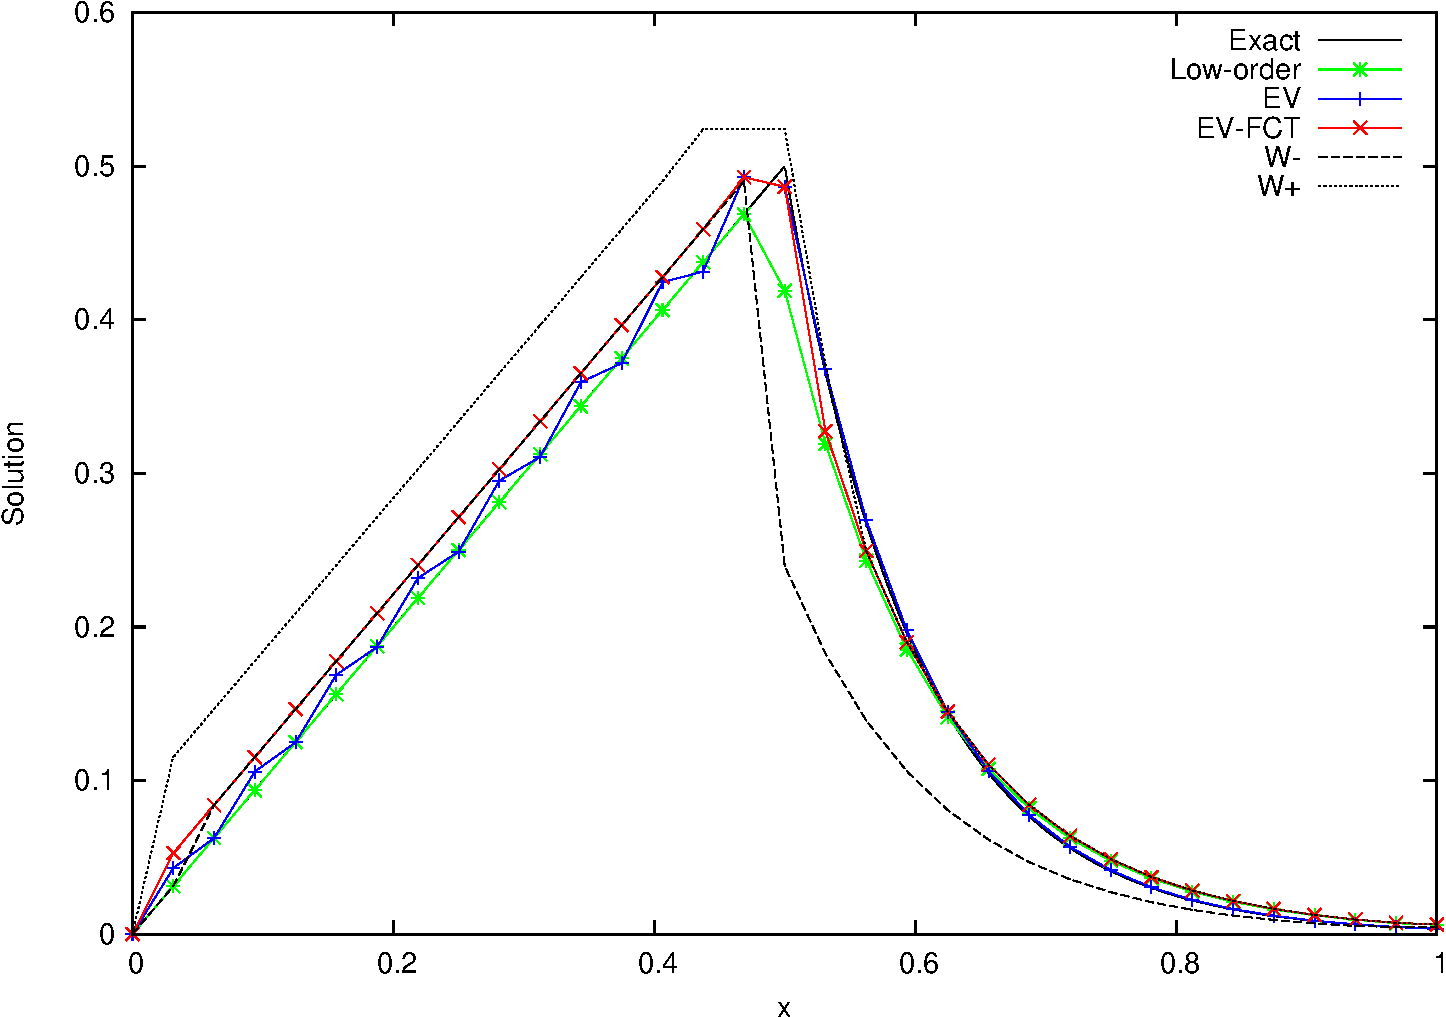
\includegraphics[height=0.8\textheight]{./figures/sourcevoid_strong1.pdf}
\end{center}

\end{frame}
%%%%%%%%%%%%%%%%%%%%%%%%%%%%%%%%%%%%%%%%%%%%%%%%%%%%%%%%%%%%%%%%%%%%%%%%%%%%%%%%%
\begin{frame}
\frametitle{Source-Void-to-Absorber Test Problem}
\framesubtitle{Strongly Imposed Dirichlet BC, $L^+=L^-=0$, SS}

\begin{center}
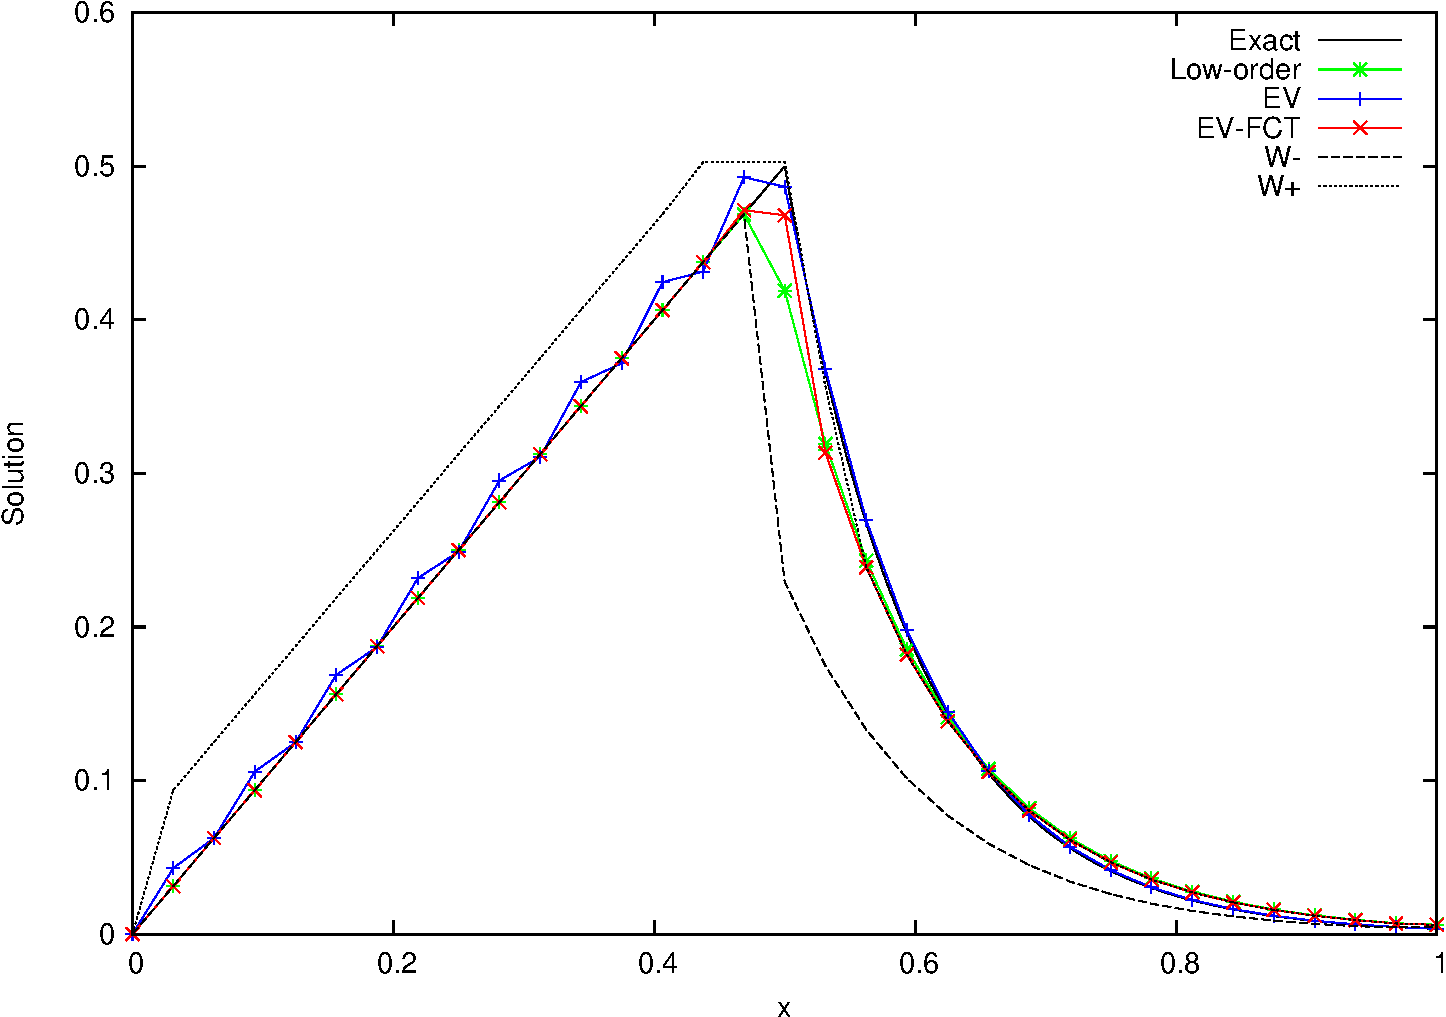
\includegraphics[height=0.8\textheight]{./figures/sourcevoid_strong0.pdf}
\end{center}

\end{frame}
%%%%%%%%%%%%%%%%%%%%%%%%%%%%%%%%%%%%%%%%%%%%%%%%%%%%%%%%%%%%%%%%%%%%%%%%%%%%%%%%%
\begin{frame}
\frametitle{Source-Void-to-Absorber Test Problem}
\framesubtitle{Number of Cells vs. Iterations Study, Backward Euler, CFL = 1}

\begin{center}
\begin{table}[h]
\caption{EV and FCT Iterations Required for EV-FCT Solution}
\begin{tabular}{c c c c c}\toprule
$N_{cell}$ & \multicolumn{2}{c}{\emph{EV}} & \multicolumn{2}{c}{\emph{FCT}}\\
           & \emph{Total} & \emph{Avg.}    &  \emph{Total} & \emph{Avg.}\\\midrule
  8 &  661 & 24.48 &   244 &  9.04\\
 16 &  807 & 19.21 &   655 & 15.60\\
 32 &  844 & 11.25 &  1194 & 15.92\\
 64 & 1204 &  8.72 &  2024 & 14.67\\
128 & 1752 &  6.59 &  3675 & 13.82\\
256 & 2713 &  5.20 &  6673 & 12.78\\
512 & 4284 &  4.14 & 12098 & 11.69\\
\bottomrule\end{tabular}
\end{table}
\end{center}

\end{frame}
%%%%%%%%%%%%%%%%%%%%%%%%%%%%%%%%%%%%%%%%%%%%%%%%%%%%%%%%%%%%%%%%%%%%%%%%%%%%%%%%%
\begin{frame}
\frametitle{Source-Void-to-Absorber Test Problem}
\framesubtitle{CFL Number vs. Iterations Study, Backward Euler, 128 cells}

\begin{center}
\begin{table}[h]
\caption{EV and FCT Iterations Required for EV-FCT Solution}
\begin{tabular}{c c c c c c c }\toprule
 & & \multicolumn{2}{c}{\emph{EV}}
  & \multicolumn{2}{c}{\emph{FCT}} &\\
\emph{CFL} & $N_{step}$ & \emph{Total} & \emph{Avg.}
  & \emph{Total} & \emph{Avg.} & $L^2$ \emph{err.}\\\midrule
0.1 & 2661 & 15006 &  5.64 & 14036 &   5.27 & $3.013\times10^{-3}$\\
0.5 &  533 &  3445 &  6.46 &  5000 &   9.38 & $3.033\times10^{-3}$\\
1.0 &  266 &  1752 &  6.59 &  3675 &  13.82 & $3.023\times10^{-3}$\\
5.0 &   54 &   471 &  8.72 & 12208 & 226.07 & $2.979\times10^{-3}$\\
10.0 &  27 &   232 &  8.59 &  6126 & 226.89 & $3.325\times10^{-3}$\\
20.0 &  14 &   133 &  9.50 &  3713 & 265.21 & $3.727\times10^{-3}$\\
50.0 &   6 &    62 & 10.33 &  2077 & 346.17 & $7.191\times10^{-3}$\\
\bottomrule\end{tabular}
\end{table}
\end{center}

\end{frame}
